\setcounter{chapter}{-1}
\chapter{Preliminaries}

\begin{prop}
    Let $M$ be a simply connected $(G,X)$-manifold. Then there exists a $(G,X)$-map
    $$
        dev: M \mapsto X
    $$
\end{prop}
\begin{proof}
    We pick a base point $x_0 \in M$ and a chart $(U_0, \varphi_0)$ around $x_0$. Now for any $x \in M$ we define the map $dev$ as follows. We pick a curve on $M$ $x(t)$ satisfying $x(0)=x_0$ and $x(1)=x$. As the image of our curve is compact, we can cover the it by finitely many coordinate charts $U_i$ with $i\in \{0, \dots,n\}$ such that $x(t) \in U_i$ for $t\in(a_i, b_i)$ with
    $$a_0<0<a_1<b_0<a_2<b_1<a_3 \dots <a_n<b_{n-1}<1<b_n$$

    \begin{center}
        \begin{marginfigure}
            \vspace{8px}
            \centering
            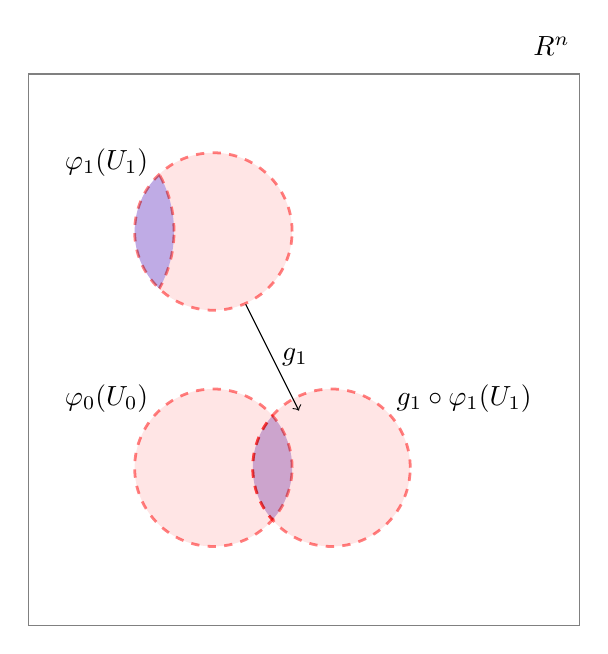
\begin{tikzpicture}
                \begin{scope}
                    \begin{scope}
                        \draw[color=black!50] (0,0) rectangle (7,7) node[color=black,anchor=east, yshift=10pt]{$\mathbb{R}^n$};
                    \end{scope}
                    \begin{scope}[transparency group]
                        \begin{scope}[blend mode=multiply, yshift=10cm, xshift=10pt]
                            \draw[dashed, color=red!50!white, fill=red!10, opacity=1]
                            (2,-8) circle (1) node[anchor=east, xshift=-20pt, yshift = 25pt, color=black]{$\varphi_0(U_0)$};
                            \draw[dashed, color=red!50!white, fill=red!10,opacity=1] (2, -5) circle (1) node[anchor=east, xshift=-20pt, yshift = 25pt, color=black]{$\varphi_1(U_1)$};
                            \begin{scope}
                                \clip (2, -5) circle (1);
                                \draw[dashed, color=red!50!white, fill=blue!25, opacity=1]
                                (0,-5) circle (1.5);
                            \end{scope}

                            \begin{scope}
                                \clip (2, -8) circle (1);
                                \draw[dashed, color=red!50!white, fill=blue!20,opacity=1] (3.5, -8) circle (1);
                            \end{scope}
                            \draw[dashed, color=red!50!white, fill=red!10,opacity=1] (3.5, -8) circle (1) node[anchor=west, xshift=20pt, yshift = 25pt, color=black]{$g_1 \circ \varphi_1(U_1)$};

                        \end{scope}
                    \end{scope}
                    \node[] (GluingOneTwoStart) at (2.7,4.2) {};
                    \node[] (GluingOneTwoEnd) at (3.5,2.6) {};
                    \path[->]
                    (GluingOneTwoStart) edge[right] node [midway, right] {$g_{1}$} (GluingOneTwoEnd);
                \end{scope}

            \end{tikzpicture}
            \caption{Gluing together charts}
            \label{fig:placeholder}
        \end{marginfigure}
        \begin{figure}[h]
            \centering
            \begin{tikzpicture}
                \begin{scope}[transparency group]
                    \begin{scope}[blend mode=multiply]
                        \draw[color=black!50] (0,0) rectangle (8,7) node[color=black,anchor=east, yshift=10pt]{\textbf{M}};
                        \draw[dashed, color=red!50!white, fill=red!10, opacity=1]
                        (1,1.8) circle (0.8) node[anchor=east, xshift=-10pt, yshift = 25pt, color=black]{$U_0$};
                        \draw[dashed, color=red!50!white, fill=red!10,opacity=1] (2, 2.5) circle (0.8) node[anchor=east, xshift=10pt, yshift = 30pt, color=black]{$U_1$};
                        \draw[-, dotted, thick] (2.8,3.5) arc (140:90:4cm and 3cm);
                        \draw[dashed, color=red!50!white, fill=red!10,opacity=1] (7, 4.7) circle (0.8) node[anchor=east, xshift=10pt, yshift = 30pt, color=black]{$U_n$};
                    \end{scope}
                \end{scope}
                \draw [cyan, yshift=-1.3cm, thick] plot [smooth, tension=1] coordinates { (1, 3) (3, 4.5) (6, 5) (7, 6)} node[color=black] at (4.5,4.5) {$x(t)$};
                \node[yshift=-1.3cm, draw, circle, fill=black!50, inner sep=1pt] (start) at (1,3) {} node[right = of start, xshift=-30pt, yshift=-5pt]{$x_0$};
                \node[yshift=-1.3cm, draw, circle, fill=black!50, inner sep=1pt] (end) at (7,6) {} node[right = of end, xshift=-30pt, yshift=-5pt]{$x$};
            \end{tikzpicture}
            \caption{Covering of $x(t)$ by charts}
            \label{fig:placeholder}
        \end{figure}
    \end{center}

    Now we consider where these charts overlap. Since our manifold is equipped with
    a $(G,X)$-structure our transition maps differ by an element of $G$. Let $g_i =
        \varphi_{i-1}\circ\varphi^{-1}_i \in G$ be the transition map from $U_i$ and
    $U_{i-1}$. We then define $$ dev(x) = g_1g_2\dots g_n \varphi_n(x) $$ We must
    show that this is a well-defined map. We first show that this map does not
    change if we refine the cover. Suppose we insert a chart $(V, \phi)$ between
    $U_i$ and $U_{i-1}$. Let
    \begin{center}
        $\varphi_{i-1} = h_{i-1}\circ\phi$ on $V \cap U_{i-1}$ and \\
        $\phi = h_i\varphi_{i}$ on $V \cap U_{i-1}$.
    \end{center}
    Then on $V \cap U_i \cap U_{i-1}$ we have that $\varphi_{i-1} = h_{i-1}\circ h_i \circ \varphi_{i}$. This gives us that $g_i = \varphi_{i-1}\circ \varphi^{-1}_i = h_{i-1} \circ h_i$ as we require that our transition maps satisfy a unique extension property.

    Now when we develop along our curve with respect to this new covering, we
    obtain that:

    \begin{center}
        $dev(x) = g_1 \dots g_{i-1}h_{i-1}h_{i}g_{i+1}\dots g_n\varphi_n(x) = g_1 \dots g_{i-1}g_ig_{i+1}\dots g_n\varphi_n(x)$
    \end{center}

    This defines $dev$ along $x(t)$. We now need to show that it does not depend on
    our choice of curve. As $M$ is simply connected, all curves with the same start
    point and end point will be homotopic. Indeed, by compactness we can split our
    homotopy into smaller homotopies such that we can break up our curve into
    regions
    \begin{center}
        $a_1 =0 < a_2 < \dots < a_n=1$
    \end{center}
    such that during each small homotopy the segment $x((a_i, a_{i+1}))$ lies entirely inside a coordinate patch. It then follows that $dev$ is independent of our choice of paths completing the proof.

\end{proof}